\section{Methodology}
\label{sec:methodology}

\subsection{Data Source}

The publicly available Emotion Dataset from Kaggle~\citep{emotions_kaggle} was utilised, a large-scale collection of Twitter posts annotated into six discrete emotion categories: anger, joy, sadness, fear, surprise, and love. The dataset comprises 416,809 labelled text samples, making it statistically robust for supervised multi-class classification.

The dataset is justified on three grounds. First, its large sample size enhances statistical reliability and reduces variance in model estimation. Second, it reflects informal, real-world social media language --- including abbreviations, emotive expressions, and conversational tone --- thereby increasing ecological validity. Third, its six-class taxonomy enables fine-grained emotional analysis beyond binary sentiment polarity, directly aligning with the research objective of multi-class emotion prediction.

Each instance consists of a raw textual input (\texttt{text}) and a corresponding encoded emotion label (\texttt{label}). Table~\ref{tab:data_dict} presents the data dictionary.

\begin{table}[H]
\centering
\caption{Data dictionary --- Kaggle Emotions Dataset.}
\label{tab:data_dict}
\footnotesize
\begin{tabular}{@{}llll@{}}
\toprule
\textbf{Column} & \textbf{dtype} & \textbf{Role} & \textbf{Description} \\
\midrule
\texttt{index} & int & Index & Row identifier \\
\texttt{text} & object & Input & Raw Twitter post text \\
\texttt{label} & int64 & Target & Encoded emotion class \\
\bottomrule
\end{tabular}
\end{table}

The label encoding follows: 0\,=\,Sadness, 1\,=\,Joy, 2\,=\,Love, 3\,=\,Anger, 4\,=\,Fear, 5\,=\,Surprise. Table~\ref{tab:sample_records} presents five representative records drawn from the dataset. Some labels may appear counter-intuitive (\eg, ``helpless'' labelled as Fear rather than Sadness), reflecting the subjective nature of crowd-sourced annotation --- a known limitation discussed in Section~\ref{sec:results}.

\begin{table}[!htb]
\centering
\caption{Sample records from the Kaggle Emotions Dataset.}
\label{tab:sample_records}
\scriptsize
\setlength{\tabcolsep}{3pt}
\begin{tabular}{@{}clc@{}}
\toprule
\textbf{Idx} & \textbf{Text (sample content)} & \textbf{Label} \\
\midrule
0 & i feel really helpless and heavy hearted & 4 (Fear) \\
1 & ive enjoyed being able to slouch about\ldots & 0 (Sadness) \\
2 & i gave up my internship\ldots feeling lost & 4 (Fear) \\
3 & i dont know i feel so lost & 0 (Sadness) \\
4 & i am a kindergarten teacher\ldots dedicated & 4 (Fear) \\
\bottomrule
\end{tabular}
\end{table}

\subsection{Exploratory Data Analysis}

Figure~\ref{fig:class_dist} and Table~\ref{tab:class_dist} show the class distribution. Joy and Sadness together account for nearly 63\% of all samples, while Surprise represents fewer than 4\% (imbalance ratio $\approx$ 9.5\,:\,1), motivating the downsampling strategy.

\begin{figure}[!htb]
\centering
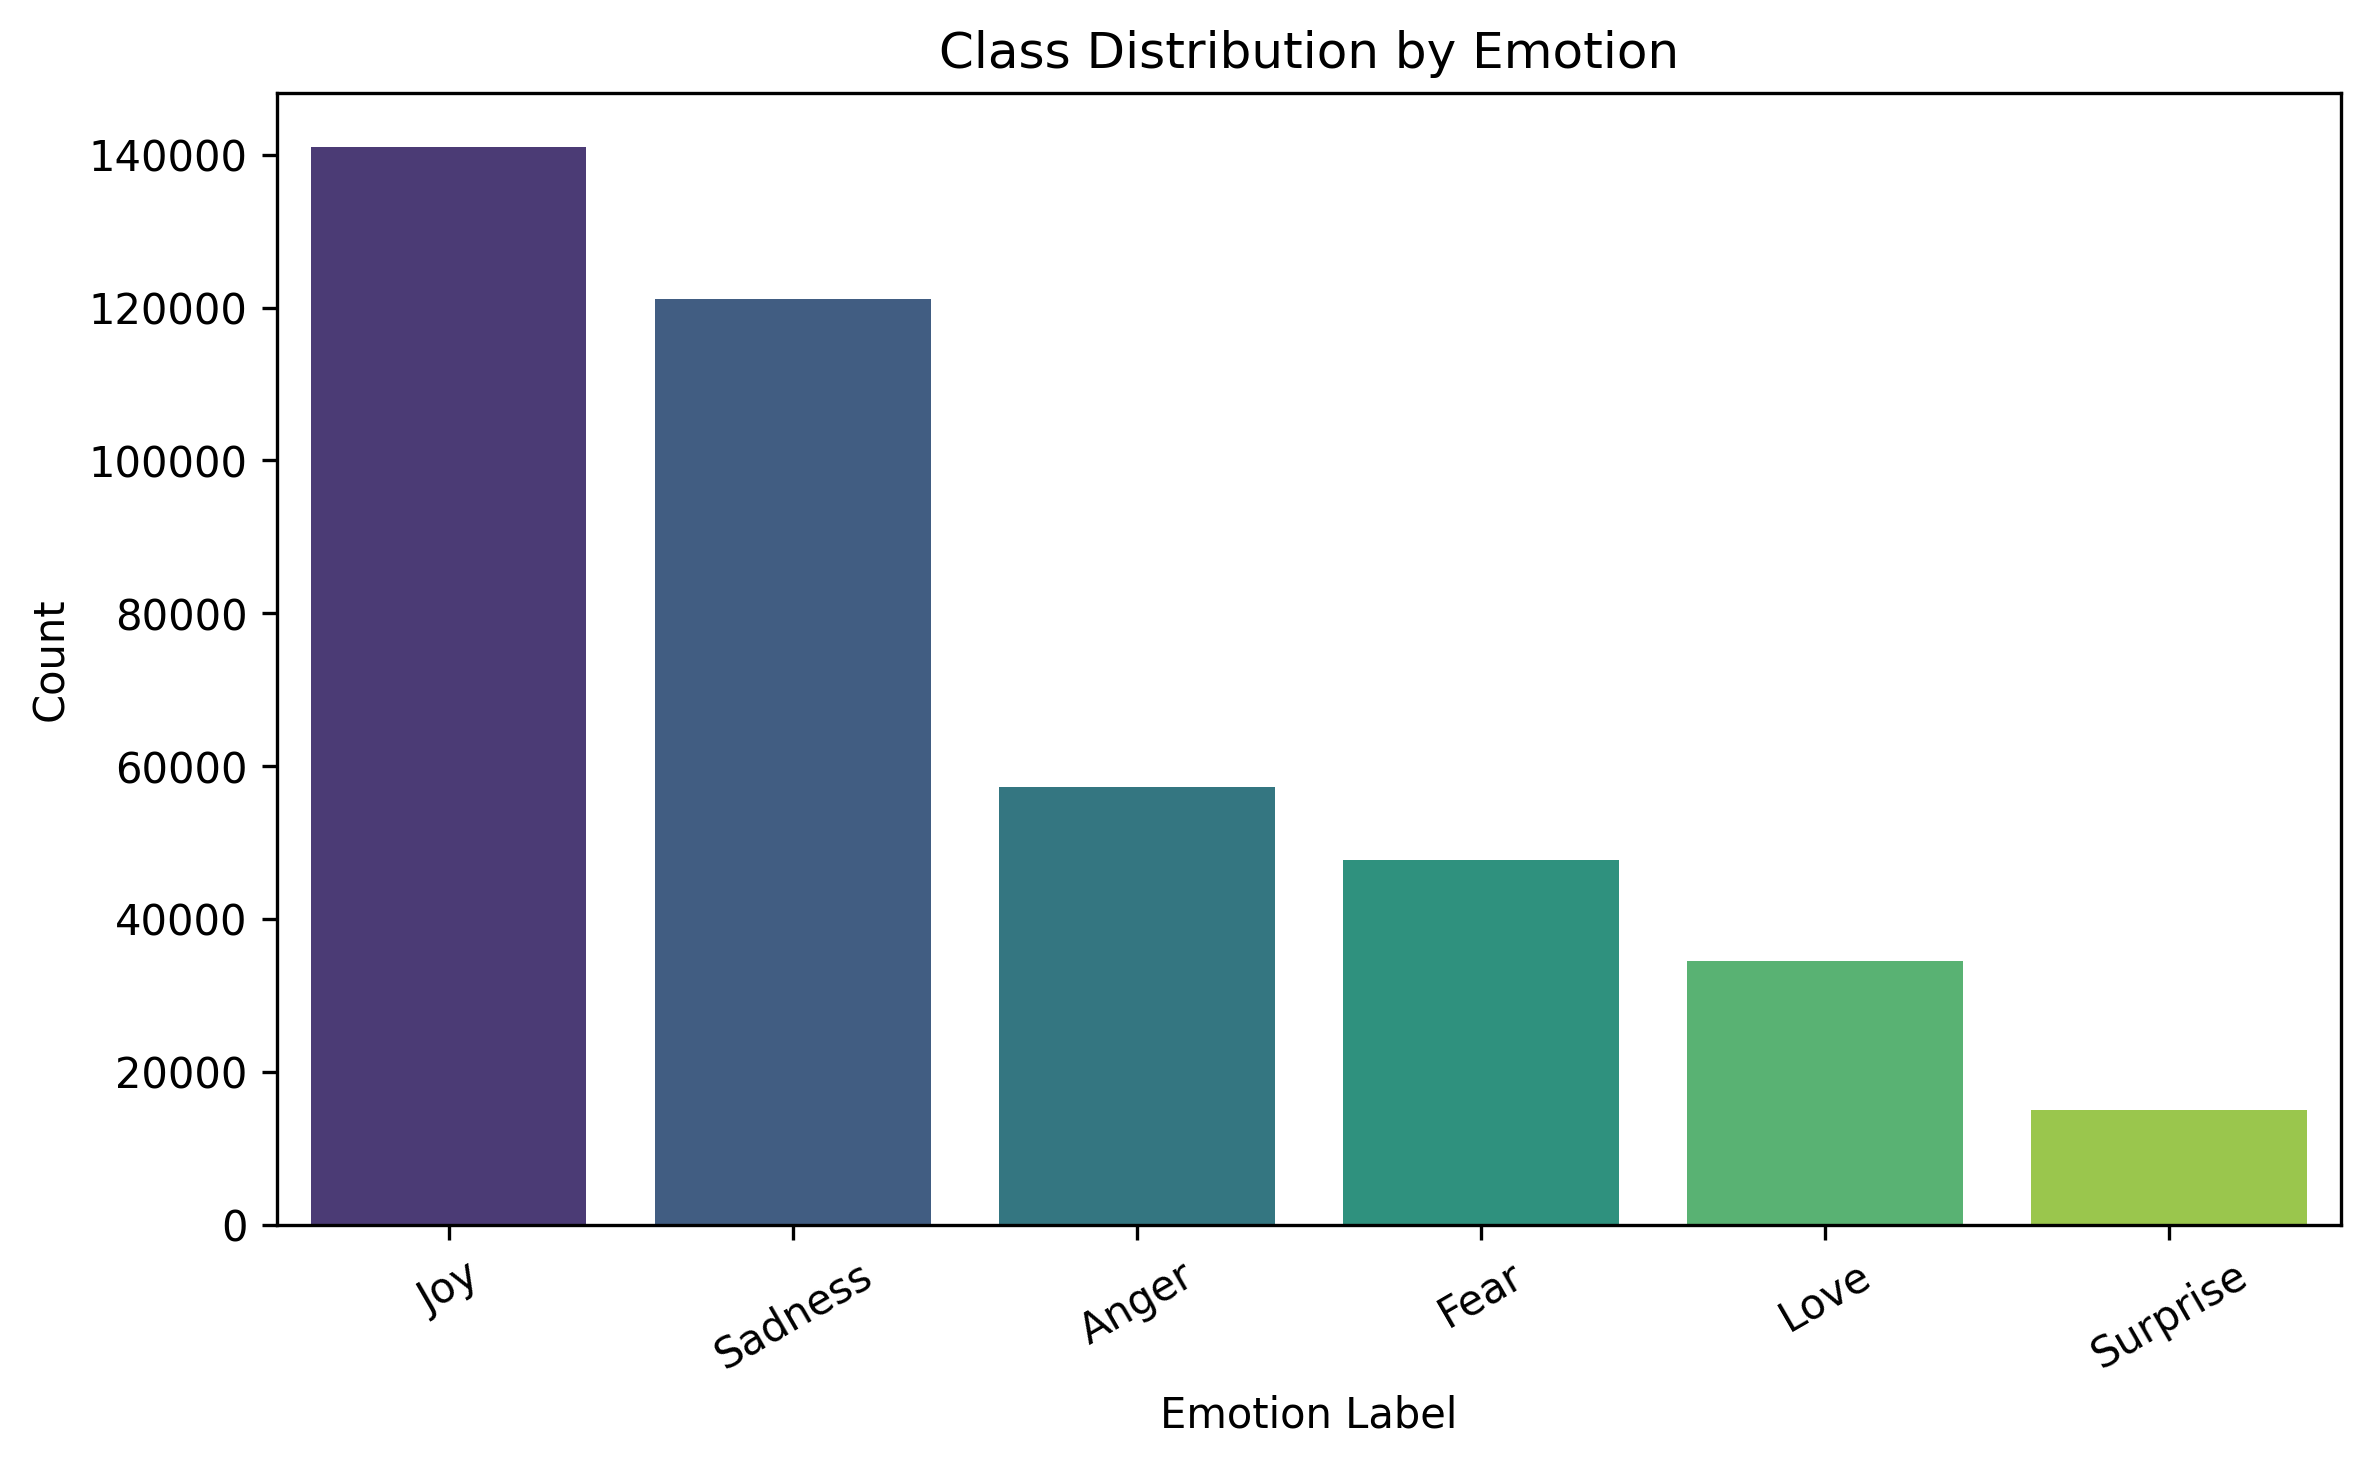
\includegraphics[width=0.82\linewidth]{figures/class_distribution.png}
\vspace{-4pt}
\caption{Class distribution by emotion label. Joy dominates at 33.8\%, while Surprise is the smallest class at 3.6\%.}
\label{fig:class_dist}
\end{figure}

\begin{table}[!htb]
\centering
\caption{Target variable distribution --- emotion class frequencies.}
\label{tab:class_dist}
\footnotesize
\begin{tabular}{@{}clrrl@{}}
\toprule
\textbf{Code} & \textbf{Emotion} & \textbf{Count} & \textbf{\%} & \textbf{Note} \\
\midrule
1 & Joy & 141{,}067 & 33.84 & Largest class \\
0 & Sadness & 121{,}187 & 29.07 & Second largest \\
3 & Anger & 57{,}317 & 13.75 & Mid-tier \\
4 & Fear & 47{,}712 & 11.45 & Overlap w/ Surprise \\
2 & Love & 34{,}554 & 8.29 & Minority class \\
5 & Surprise & 14{,}972 & 3.59 & Highest misclass.\ risk \\
\midrule
  & \textbf{Total} & \textbf{416{,}809} & & \\
\bottomrule
\end{tabular}
\end{table}

Table~\ref{tab:eda_summary} summarises per-class text length statistics. Posts are concentrated between 20--150 characters (right-skewed), with Love producing the longest posts (median 94 chars) and Anger the shortest (median 84). These statistics informed maximum sequence length and padding strategies for DL models. A Pearson correlation analysis confirmed strong redundancy between \texttt{text\_length} and \texttt{word\_count} ($r = 0.984$), while correlation between label encoding and length features was near-zero ($r < 0.03$), confirming that classification depends on semantic content rather than message length. Full distribution plots are in Appendix~\ref{sec:appendix} (Figure~\ref{fig:text_length}).

\begin{table}[!htb]
\centering
\caption{Per-class text length statistics (characters).}
\label{tab:eda_summary}
\footnotesize
\setlength{\tabcolsep}{3pt}
\begin{tabular}{@{}lrrrr@{}}
\toprule
\textbf{Emotion} & \textbf{Min} & \textbf{Max} & \textbf{Mean} & \textbf{Median} \\
\midrule
Joy       & 2 & 465 & 93.4 & 85 \\
Sadness   & 2 & 493 & 99.2 & 88 \\
Anger     & 2 & 478 & 94.8 & 84 \\
Fear      & 3 & 487 & 101.6 & 90 \\
Love      & 3 & 471 & 104.3 & 94 \\
Surprise  & 3 & 459 & 98.7 & 87 \\
\midrule
\textbf{Overall} & 2 & 493 & 97.0 & 86 \\
\bottomrule
\end{tabular}
\end{table}

\subsection{System Architecture}

The methodology followed a structured NLP workflow: preprocessing $\rightarrow$ feature extraction $\rightarrow$ model development $\rightarrow$ evaluation $\rightarrow$ deployment. The full pipeline is illustrated in Figure~\ref{fig:pipeline}.

\textbf{Preprocessing.} An eight-step NLP pipeline normalised raw text prior to feature extraction. Table~\ref{tab:preproc_steps} details each step and its rationale. Stopword removal used the NLTK English stopword list; however, negation words and intensifiers (\eg, ``not'', ``never'', ``very'', ``extremely'') were retained via a custom exception list, as these tokens carry direct emotional polarity and their removal would cause loss of discriminative signal. Class imbalance was addressed through random downsampling to the minority-class size ($\approx$14,972 per class, 89,832 total). Downsampling was chosen for experimental simplicity and to ensure equal class representation; however, it discards approximately 78\% of the data, and alternatives such as class weighting or SMOTE may yield better generalisation.

\begin{table}[!htb]
\centering
\caption{Eight-step NLP preprocessing pipeline.}
\label{tab:preproc_steps}
\footnotesize
\setlength{\tabcolsep}{3pt}
\begin{tabular}{@{}cll@{}}
\toprule
\textbf{\#} & \textbf{Step} & \textbf{Rationale} \\
\midrule
1 & Lowercasing & Normalise case variance \\
2 & Whitespace stripping & Remove extra spaces \\
3 & URL removal & Discard non-textual noise \\
4 & Emoji removal & Remove non-alphabetic symbols \\
5 & Special char.\ removal & Retain only \texttt{[a-z\textbackslash s]} \\
6 & Chat-word expansion & Expand 31 abbreviations \\
7 & Stopword removal & Remove noise; retain negations \\
8 & Lemmatisation & Reduce morphological variants \\
\bottomrule
\end{tabular}
\end{table}

\begin{figure}[H]
\centering
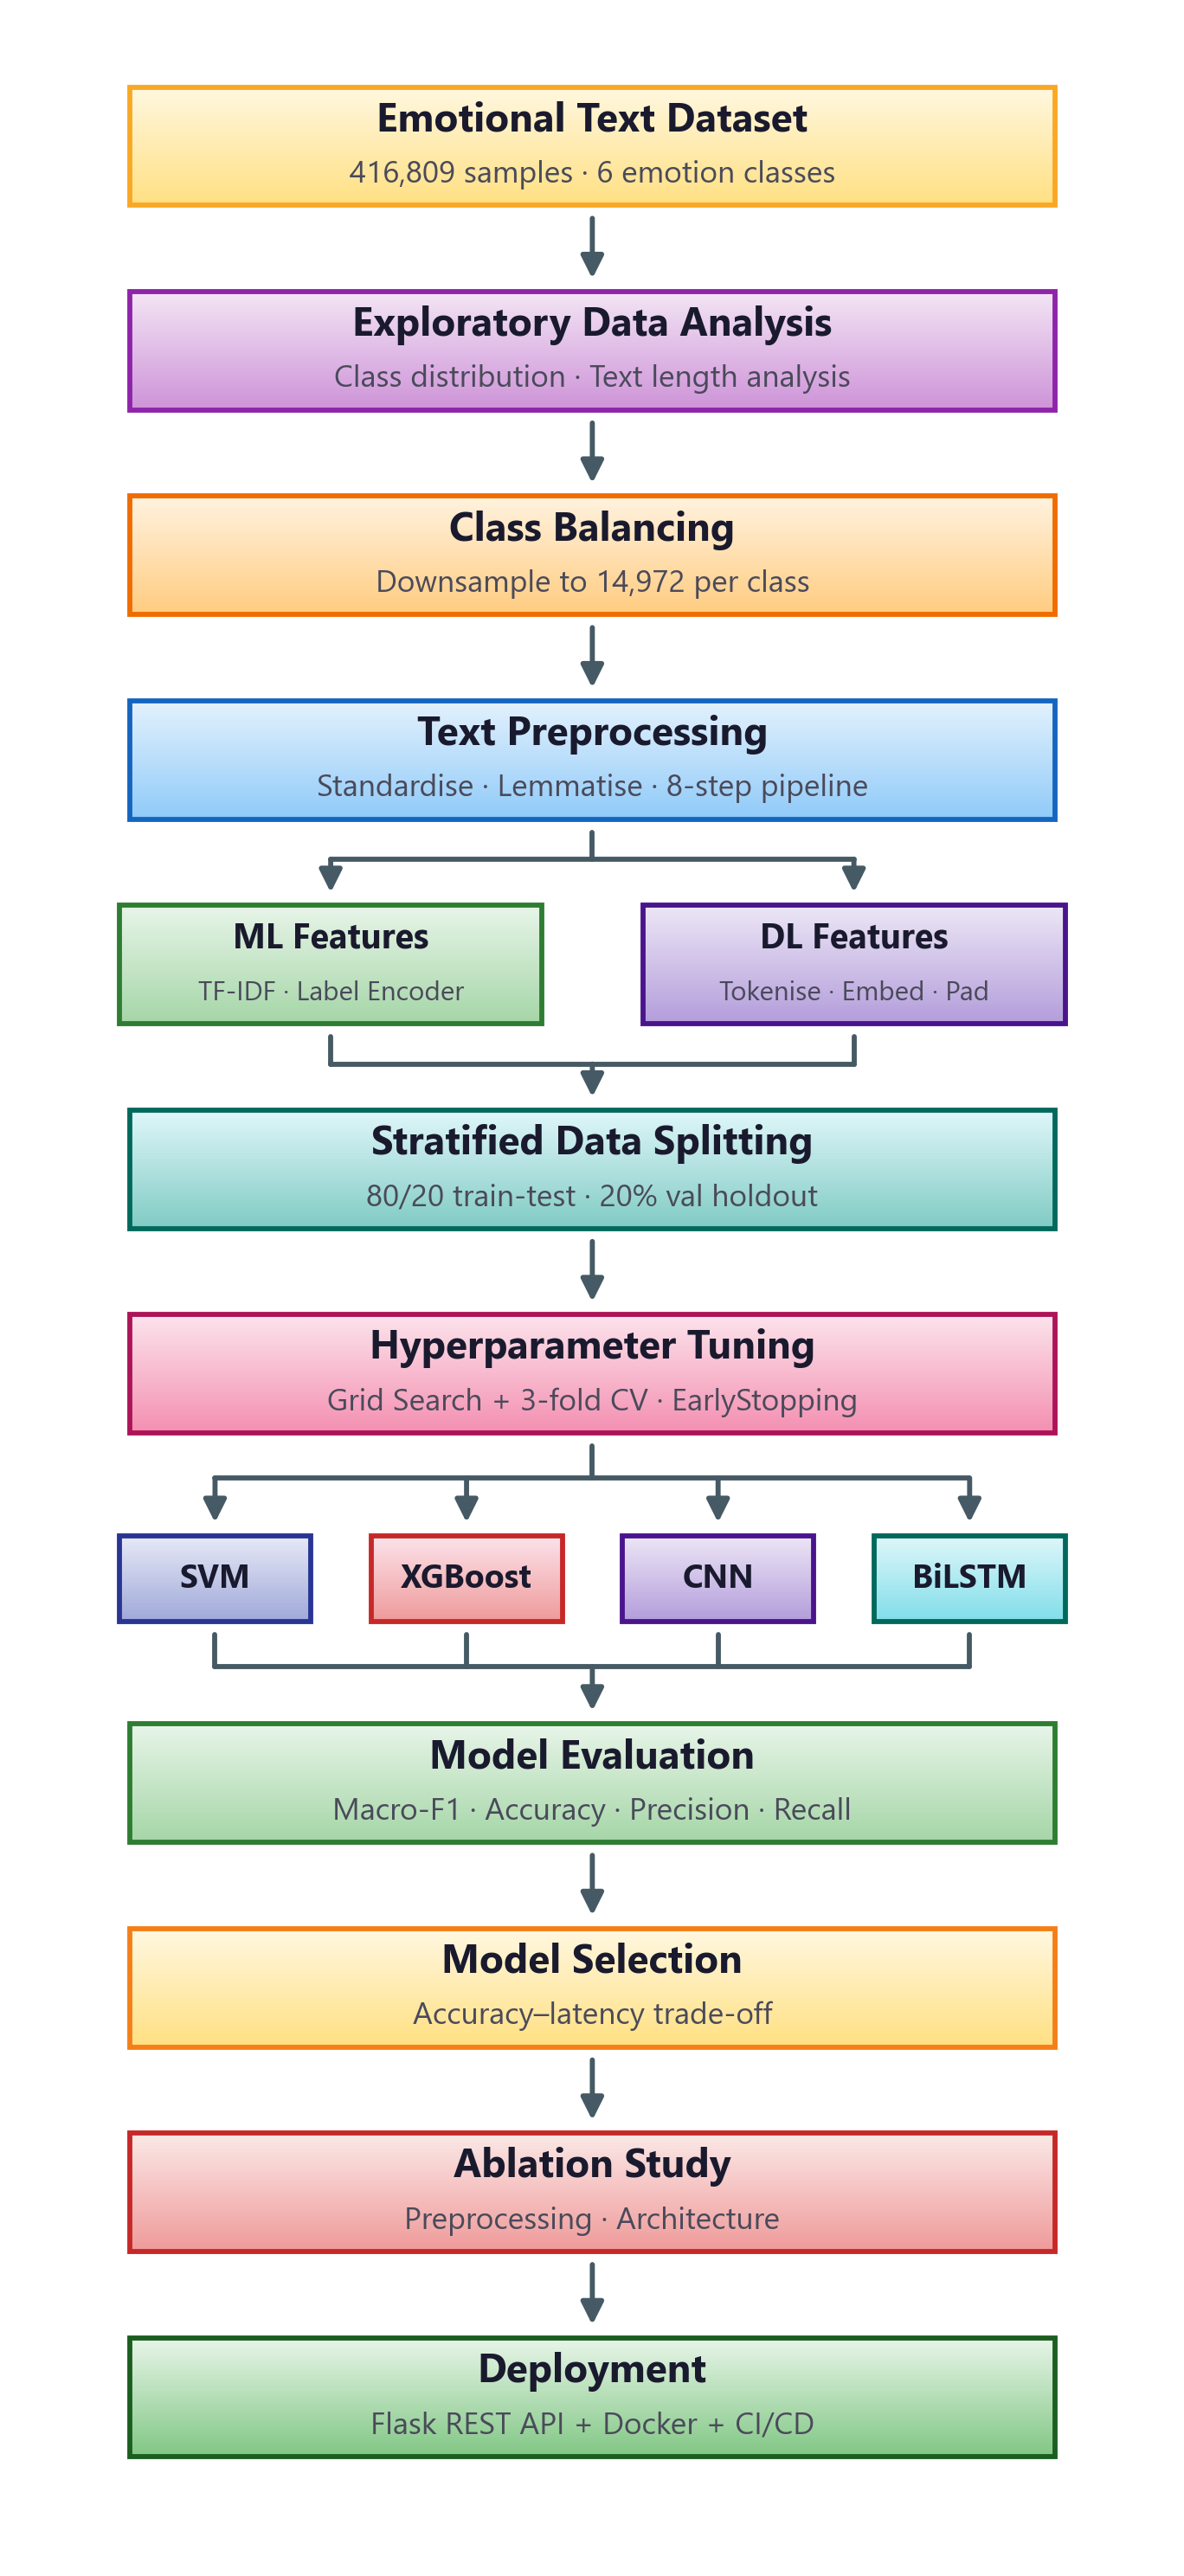
\includegraphics[width=0.75\linewidth]{img/processflow.png}
\caption{MindTrace end-to-end pipeline architecture.}
\label{fig:pipeline}
\end{figure}

\textbf{Feature Representation.} Table~\ref{tab:feat_eng} compares the feature engineering strategies for ML and DL model families. For machine learning models, TF-IDF vectorisation (\texttt{max\_features=5000}, \texttt{ngram\_range=(1,2)}) transforms text into numerical representations capturing both unigrams and bigrams:

\begin{table}[!htb]
\centering
\caption{Feature engineering comparison --- ML vs.\ DL pipelines.}
\label{tab:feat_eng}
\footnotesize
\setlength{\tabcolsep}{3pt}
\begin{tabular}{@{}lll@{}}
\toprule
\textbf{Aspect} & \textbf{ML (SVM, XGBoost)} & \textbf{DL (CNN, BiLSTM)} \\
\midrule
Method      & TF-IDF vectorisation      & Trainable embedding \\
Vocab size  & 5{,}000 features          & 60{,}000 tokens \\
N-grams     & (1,\,2)                   & N/A (learned) \\
Dim.        & 5{,}000 (sparse)          & 100 (dense) \\
Seq.\ info  & Lost (bag-of-words)       & Preserved (padding) \\
\bottomrule
\end{tabular}
\end{table}
\begin{equation}
\text{TF-IDF}(t, d) = \text{TF}(t, d) \times \log\!\left(\frac{N}{\text{DF}(t)}\right)
\label{eq:tfidf}
\end{equation}
where $\text{TF}(t,d)$ is the term frequency, $\text{DF}(t)$ is the document frequency, and $N$ is the total number of documents. For deep learning models, an embedding layer converts tokens into dense vector representations.

\textbf{Data Splitting.} The dataset was split 80\% training / 20\% testing with a 20\% validation holdout from training data, using stratified sampling to preserve class proportions. After downsampling (89,832 total samples), this yielded 57,492 training, 14,373 validation, and 17,967 test samples.

\textbf{Evaluation Metrics.} Model performance was evaluated using precision, recall, per-class F1, macro-averaged F1 ($K=6$ classes), and accuracy:
\begin{align}
\text{Precision} &= \frac{TP}{TP + FP} \label{eq:precision}\\
\text{Recall} &= \frac{TP}{TP + FN} \label{eq:recall}\\
F_1 &= \frac{2 \times \text{Precision} \times \text{Recall}}{\text{Precision} + \text{Recall}} \label{eq:f1}\\
\text{Macro-}F_1 &= \frac{1}{K}\sum_{k=1}^{K} F_{1,k} \label{eq:macro_f1}\\
\text{Accuracy} &= \frac{\text{Number of correct predictions}}{\text{Total predictions}} \label{eq:accuracy}
\end{align}
